\documentclass[12pt]{article}
\usepackage{preamble}

\pagestyle{fancy}
\fancyhead[LO,LE]{Теория вероятности}
\fancyhead[CO,CE]{17.09.2024}
\fancyhead[RO,RE]{Лекции Блаженова А. В.}

\fancyfoot[L]{\scriptsize исходники найдутся тут: \\ \url{https://github.com/pelmesh619/itmo_conspects} \Cat}

\begin{document}
    \section{Лекция 3}

    \subsection{Условная вероятность}

    Условная вероятность $P(A|B)$ (или $P_B(A)$) - вероятность события $A$, вычисленная в предположении, что событие $B$ уже произошло

    \Ex Бросается кость один раз, известно, что выпало больше 3 очков. Найти вероятность того, что выпало четное число очков

    \smallvspace

    \begin{minipage}{\linewidth}
        \begin{wrapfigure}{r}{0pt}
            \begin{center}
                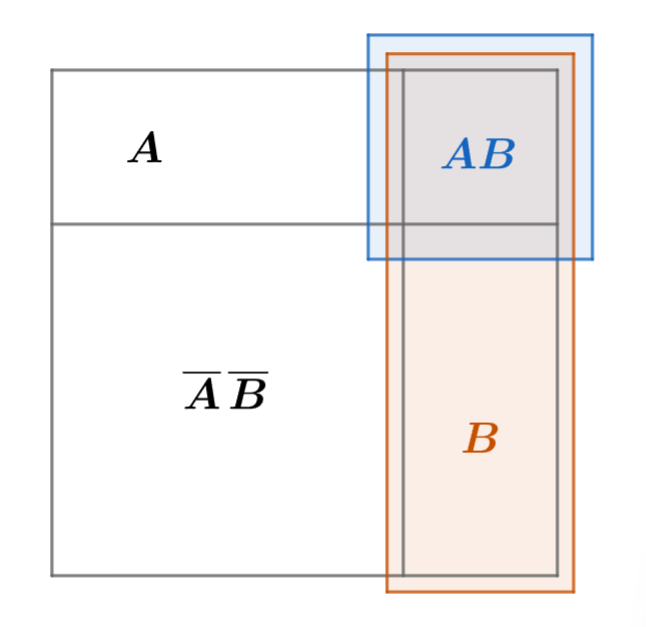
\includegraphics[height=5cm]{probtheory/images/probtheory_2024_09_17_1}
            \end{center}
        \end{wrapfigure}

        $A$ - выпало четное число очков

        $B$ - выпало больше трех очков

        $\Omega = \{1, 2, 3, 4, 5, 6\}; |\Omega| = 6; A = \{2, 4, 6\}; B = \{4, 5, 6\}$

        $P(A|B) = \frac{2}{3} = \frac{\frac{2}{6}}{\frac{3}{6}} = \frac{P(AB)}{P(B)}$


        Интерпретация с помощью геометрической вероятности:

        $P(A|B) = \frac{S_{AB}}{S_B} = \frac{\frac{S_{AB}}{S_\Omega}}{\frac{S_B}{S_\Omega}}$
    \end{minipage}

    \Def Условной вероятностью события $A$ при условии, что имело место событие $B$, называется величина $P(A|B) = \frac{P(AB)}{P(B)}$

    \Ex Известно, что среди населения 1\% воров. В комнате, где находилось 10 гостей, у хозяина пропал кошелек. Какова вероятность того, что произвольный гость является вором.

    $A$ - гость является вором $P(A) = 0.01$

    $B$ - пропал кошелек (хотя бы один вор среди гостей есть)

    $P(A|B) = \frac{P(AB)}{P(B)} = \frac{P(AB)}{1 - P(\overline{B})} = \frac{P(A)}{1 - 0.99^{10}} = \frac{0.01}{1 - 0.99^{10}} = 0.105$

    Формула умножения:

    В качестве следствия условной вероятности получаем:

    $P(A|B) = \frac{P(AB)}{P(B)} \Longrightarrow P(AB) = P(B) \cdot P(A|B) = P(A) \cdot P(B|A)$

    Общий случай:

    $P(A_1 A_2 A_3 \dots A_n) = P(A_1) P(A_2 | A_1) P(P_3 | A_1 A_2) \dots P(A_n | A_1 A_2 \dots A_{n - 1})$

    \begin{tcolorbox}
        $\Box$

        База индукции $P(AB) = P(B) P(A|B)$

        Шаг индукции: пусть верно при $n - 1$:

        $P(A_1 A_2 A_3 \dots A_{n - 1}) = P(A_1) P(A_2 | A_1) P(P_3 | A_1 A_2) \dots P(A_n | A_1 A_2 \dots A_{n - 2})$

        $P(A_1 A_2 A_3 \dots A_n) = P(A_1 A_2 A_3 \dots A_{n - 1}) \cdot P(A_n | A_1 A_2 \dots A_{n - 1}) = \\
        P(A_1) P(A_2 | A_1) P(P_3 | A_1 A_2) \dots P(A_n | A_1 A_2 \dots A_{n - 1})$

        $\Box$
    \end{tcolorbox}


    \Ex Студент выучил 1 билет из $n$, в группе $n$ студентов. Каким по очереди ему нужно зайти, чтобы вероятность сдать экзамен была наибольшей

    Пусть $A_i$ - билет, вытянутый на $i$-ом шаге ($1 \leq i \leq n$)

    $A$ - студент сдал экзамен

    $P(A) = P(\overline{A_1} \cdot \overline{A_2} \cdot \dots \cdot \overline{A_{i - 1}} \cdot A_i) = \frac{n - 1}{n} \cdot \frac{n - 2}{n - 1} \cdot \dots \cdot \frac{n - (i - 1)}{n - (i - 2)} \cdot \frac{1}{n - (i - 1)} = \frac{1}{n}$

    \subsection{Полная группа событий}

    \Def События $H_1, H_2, \dots, H_n, \dots$ образуют полную группу событий, если они попарно несовместны и содержат все возможные элементарные исходы

    $H_i \cap H_j = \emptyset \ \forall i, j \quad\quad\quad \bigunion_{i = 1}^{\infty} H_i = \Omega$

    Следствие: $\sum_{i = 1}^\infty P(H_i) = 1$

    \ThN{Формула полной вероятности} $\letsymbol H_1, H_2, \dots, H_n, \dots$ - полная группа событий. Тогда $P(A) = \sum_{i = 1}^\infty P(H_i) P(A | H_i)$

    \begin{tcolorbox}
        $\Box$

        $P(A) = P(\Omega A) = P((H_1 + H_2 + H_3 + \dots) A) = P(H_1 A + H_2 A + H_3 A + \dots) = [H_i \cdot A \cdot H_j \cdot A = \emptyset \cdot A] = P(H_1 A) + P(H_2 A) + \dots =
        P(H_1) P(A | H_1) + P(H_2) P(A | H_2) + \dots$

        $\Box$
    \end{tcolorbox}

    \ThN{Формула Байеса} $\letsymbol H_1, H_2, \dots, H_n$ - полная группа событий, и известно, что событие $A$ уже произошло

    Тогда $P(H_k | A) = \frac{P(H_k) P(A | H_k)}{\sum_{i = 1}^\infty P(H_i) P(A | H_i)}$

    \begin{tcolorbox}
        $\Box$

        $P(H_k | A) = \frac{P(H_k A)}{P(A)} = \frac{P(H_k) P(A|H_k)}{\sum_{i = 1}^\infty P(H_i) P(A|H_i)}$

        $\Box$
    \end{tcolorbox}

    \ExN{1} В первой коробке 4 белых и 2 черных шара, во второй 1 белый и 2 черных. Из первой коробки во вторую переложили 2 шара, затем из второй коробки достали шар. Какова
    вероятность того, что он оказался белым

    $\letsymbol H_1$ - переложили 2 белых
    $H_2$ - 2 черных

    $H_3$ - разного цвета

    $A$ - из второй коробки достали белый шар

    $P(H_1) = \frac{4}{6} \cdot \frac{3}{5} = \frac{6}{15}$

    $P(H_2) = \frac{2}{6} \cdot \frac{1}{5} = \frac{1}{15}$

    $P(H_3) = \frac{4}{6} \cdot \frac{2}{5} + \frac{2}{6} \cdot \frac{4}{5} = \frac{4}{15} + \frac{4}{15} = \frac{8}{15}$

    $P(A) = P(H_1) \cdot P(A|H_1) + P(H_2) \cdot P(A|H_2) + P(H_3) \cdot P(A|H_3) = \frac{6}{15} \cdot \frac{3}{5} + \frac{1}{15} \cdot \frac{1}{5} + \frac{8}{15} \cdot \frac{2}{5} =
    \frac{18}{75} + \frac{1}{75} + \frac{16}{75} = \frac{35}{75} = \frac{7}{15}$

    \ExN{2} Вероятность попадания первого стрелка в цель $0.9$, а второго $0.3$. Наугад вызванный стрелок попал в цель. Какова вероятность того, что это бы первый стрелок?

    $H_1$ - вызван первый стрелок

    $H_2$ - вызван второй стрелок

    $A$ - стрелок попал

    $P(H_1) = P(H_2) = \frac{1}{2}$

    $P(A|H_1) = 0.9 \quad\quad P(A|H_2) = 0.3$

    $P(H_1 | A) = \frac{P(H_1) P(A|H_1)}{P(H_1) P(A|H_1) + P(H_2) | P(A | H_2)} = \frac{\frac{1}{2} 0.9}{\frac{1}{2} 0.9 + \frac{1}{2} 0.3} = \frac{9}{9 + 3} = 0.75$

    \ExN{3} По статистике раком болеет 1\% населения. Тест дает правильный результат в 99\% случаев. Тест оказался положительный. Найти вероятность того, что человек болен.

    $H_1$ - человек болен

    $H_2$ - человек здоров

    $A$ - анализ положительный

    $P(H_1) = 0.01$

    $P(H_2) = 0.99$

    $P(A|H_1) = 0.99$

    $P(A|H_2) = 0.01$

    $P(H_1 | A) = \frac{P(H_1)P(A | H_1)}{P(H_1) P(A | H_1) + P(H_2) P(A | H_2)} = \frac{0.01 \cdot 0.99}{0.01 \cdot 0.99 + 0.99 \cdot 0.01} = \frac{1}{2} = 0.5$

    Допустим, что второй независимый с первым анализ также оказался положительным. Найти вероятность того, что человек болен.

    $P(H_1) = 0.01 \quad\quad P(H_2) = 0.99$

    $P(AA|H_1) = 0.99^2 \quad\quad P(AA|H_2) = 0.01^2$

    $P(H_1 | AA) = \frac{0.01 \cdot 0.99^2}{0.01 \cdot 0.99^2 + 0.99 \cdot 0.01^2} = \frac{0.99}{0.99 + 0.01} = 0.99$

    Интуитивно вероятность $\frac{1}{2}$ может поддаваться непониманию, однако можно рассуждать так:
    пусть в городе живут 10000 человек, из них 100 болеют, а у 99 из них положительный анализ; у других 9900 положительный анализ всего лишь у 99, отсюда выходит $\frac{1}{2}$

    \ExN{4} В телевизионной студии 3 двери {\Large 🚪🚪🚪}, за одной из них приз {\Large 🚗}.
    Игрок выбрал наугад одну из 3 дверей, после чего ведущий открывает одну из двух оставшихся дверей и показывает, что там приза нет {\Large 🛴}. После чего
    предлагает игроку поменять свой выбор. Стоит ли игроку соглашаться?

    $H_1$ - игрок угадал

    $H_2$ - игрок не угадал

    $A$ - ведущий открыл дверь без приза

    $P(H_1) = \frac{1}{3} \quad\quad P(H_2) = \frac{2}{3}$

    $P(A|H_1) = 1 \quad\quad P(A|H_2) = \frac{1}{2}$

    $P(H_1|A) = \frac{\frac{1}{3} \cdot 1}{\frac{1}{3} \cdot 1 + \frac{1}{3} \cdot \frac{1}{2}} = \frac{1}{2}$

    Но это неправильно, так как действия ведущего неслучайны - он всегда откроет дверь без приза

    В этом случае, если мы гипотетически выберем 300 дверей, в 100 случаях мы отгадаем, ведущий откроет любую дверь без приза;
    но в 200 случаях мы не отгадаем, ведущий откроет вторую дверь без приза, и в этом случае мы сможем поменяться на дверь с призом,
    отсюда шанс $\frac{2}{3}$, если мы поменяем свой выбор \hfill


    \ExN{5} Вероятность того, что в семье с детьми ровно $k$ детей, равна $\frac{1}{2^k}$, $k = 1, 2, \dots$
    Какова вероятность того, что в семье один мальчик, если известно, что нет
    девочки? Рождения мальчиков и девочек равновероятны.


    $H_i$ - в семье $i$ детей ($1 \leq i < \infty$)

    $P(H_i) = \frac{1}{2^i}$

    $A$ - в семье нет девочки

    $P(A|H_1) = \frac{1}{2}$

    $P(A|H_2) = \frac{1}{4}$

    $P(A|H_i) = \frac{1}{2^i}$

    $P(H_1 | A) = \frac{\frac{1}{2} \frac{1}{2}}{\sum_{i = 1}^\infty \frac{1}{2^i} \cdot \frac{1}{2^i}} = \frac{\frac{1}{4}}{\frac{\frac{1}{4}}{1 - \frac{1}{4}}} = \frac{3}{4} = 0.75$


\end{document}
